\appendix
\definecolor{codegreen}{rgb}{0,0.6,0}
\definecolor{codegray}{rgb}{0.5,0.5,0.5}
\definecolor{codepurple}{rgb}{0.58,0,0.82}
\definecolor{backcolour}{rgb}{0.95,0.95,0.92}

\lstdefinestyle{mystyle}{
    backgroundcolor=\color{backcolour},   
    commentstyle=\color{codegreen},
    keywordstyle=\color{magenta},
    numberstyle=\tiny\color{codegray},
    stringstyle=\color{codepurple},
    basicstyle=\ttfamily\footnotesize,
    breakatwhitespace=false,         
    breaklines=true,                 
    captionpos=b,                    
    keepspaces=true,                 
    numbers=left,                    
    numbersep=5pt,                  
    showspaces=false,                
    showstringspaces=false,
    showtabs=false,                  
    tabsize=2
}

\lstset{style=mystyle}

\label{sec:appendix}

\section{User Study}
\label{sec:appendix_user_study}

Quality responses were ensured by three separate mechanisms:
\begin{itemize}[itemsep=-1ex,partopsep=1ex,parsep=1ex]
    \item Prolific's automatic vetting, which ensures that participants whose survey responses are rejected too often are kicked from the platform.
    \item Restriction to participants from the United States, which is known to mitigate the frequency of fraudulent responses~\cite{kennedy2020shape}.
    \item Filtering out participants via identifying survey responses which incorrectly answer control questions.
    By this process, we eliminated 20 participants, resulting in a filtered total of 147 participants.
\end{itemize}

\begin{figure}
    \centering
    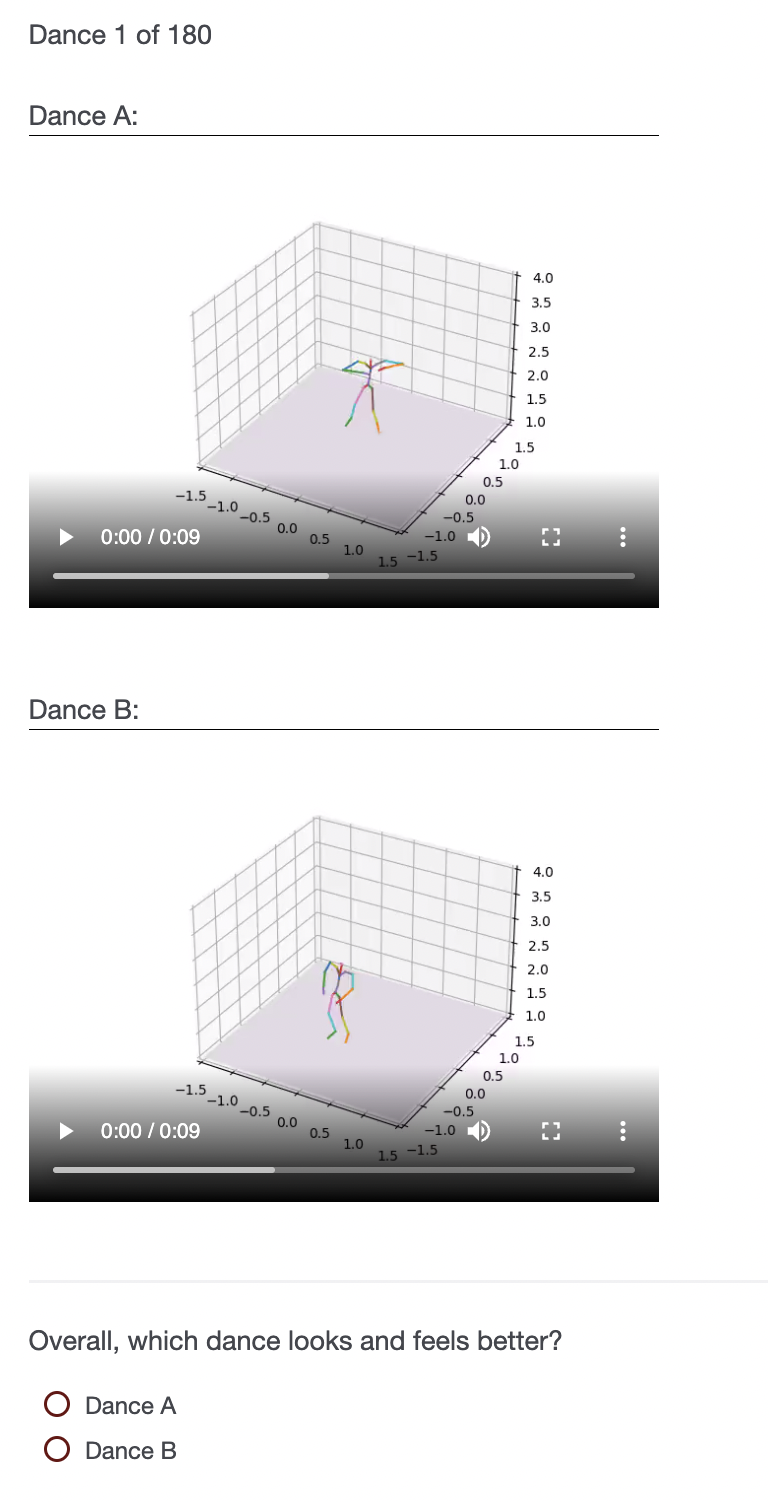
\includegraphics[width=\linewidth]{Figure6.png}
    \caption{A screenshot of the user interface from our surveys.
    We use simple stick figures as the skeleton for our dance to (1) ensure fair comparisons with \textit{Bailando}, which is difficult to rig due to the fact that it operates in Cartesian space, and (2) computational efficiency.}
    \label{fig:6}
\end{figure}

For our overall evaluations, we also evaluated against the 10 checkpoints taken throughout model training in order to increase coverage across skill levels for our Elo calculations.

In our physical plausibility survey, we ask ``Which dance is more physically plausible?'', but otherwise the survey is exactly the same.

Over the course of 24 days, we collected responses from all of the raters and plot them below in a win table. We compute our Elo and win rate metrics from this table's numbers.
Elo was computed using the \href{https://github.com/ddm7018/Elo}{Elo package} in Python by randomly sorting all matchups and obtaining the average Elo over 1000 trials.
See \cref{tab:win_table} for the raw win numbers across all of the methods we tested.

For our confidence intervals, we treated each pair of methods independently, and then each win or fail as an independent Bernoulli trial, computing the 95\% confidence interval based on the number of wins and fails for that pair (Binomial distribution).

\begin{table*}[t]
\centering
\resizebox{\textwidth}{!}{
  \begin{tabular}{lcccccccccccccccccccccccc}
    \toprule
    \textbf{Method A / Method B} & \rotatebox[origin=c]{90}{Checkpoint 200} & \rotatebox[origin=c]{90}{Checkpoint 400} & \rotatebox[origin=c]{90}{Checkpoint 600} & \rotatebox[origin=c]{90}{Checkpoint 800} & \rotatebox[origin=c]{90}{Checkpoint 1000} & \rotatebox[origin=c]{90}{Checkpoint 1200} & \rotatebox[origin=c]{90}{Checkpoint 1400} & \rotatebox[origin=c]{90}{Checkpoint 1600} & \rotatebox[origin=c]{90}{Checkpoint 1800} & \rotatebox[origin=c]{90}{Checkpoint 2000} & \rotatebox[origin=c]{90}{Ground Truth} & \rotatebox[origin=c]{90}{FACT} & \rotatebox[origin=c]{90}{EDGE (J+C' ($w=2$))} & \rotatebox[origin=c]{90}{EDGE (J+C ($w=2$))} & \rotatebox[origin=c]{90}{EDGE (J ($w=2$))} & \rotatebox[origin=c]{90}{EDGE ($w=2$)} & \rotatebox[origin=c]{90}{\textit{Bailando}} & \rotatebox[origin=c]{90}{EDGE (J+C OOD ($w=2$))} & \rotatebox[origin=c]{90}{EDGE (C OOD ($w=2$))} & \rotatebox[origin=c]{90}{EDGE (J+C ($w=1$))} & \rotatebox[origin=c]{90}{EDGE (J ($w=1$))} & \rotatebox[origin=c]{90}{EDGE (J+C' ($w=1$))} & \rotatebox[origin=c]{90}{FACT (OOD)} & \rotatebox[origin=c]{90}{\textit{Bailando} (OOD)} \\
    \midrule
    Checkpoint 200 & 0 & 3 & 3 & 3 & 1 & 2 & 0 & 1 & 0 & 0 & 1 & 0 & 0 & 0 & 0 & 1 & 0 & 0 & 1 & 0 & 0 & 0 & 0 & 0 \\
    Checkpoint 400 & 37 & 0 & 4 & 0 & 1 & 0 & 0 & 2 & 1 & 1 & 0 & 0 & 0 & 0 & 0 & 0 & 0 & 0 & 1 & 0 & 0 & 0 & 1 & 2 \\
    Checkpoint 600 & 37 & 36 & 0 & 4 & 3 & 0 & 1 & 2 & 1 & 1 & 2 & 7 & 0 & 1 & 2 & 0 & 0 & 0 & 0 & 0 & 1 & 1 & 1 & 16 \\
    Checkpoint 800 & 37 & 40 & 36 & 0 & 9 & 5 & 5 & 0 & 4 & 0 & 1 & 10 & 1 & 4 & 1 & 2 & 1 & 0 & 1 & 0 & 2 & 1 & 7 & 16 \\
    Checkpoint 1000 & 39 & 39 & 37 & 31 & 0 & 11 & 1 & 7 & 9 & 4 & 4 & 19 & 6 & 5 & 6 & 2 & 16 & 3 & 1 & 0 & 1 & 0 & 15 & 17 \\
    Checkpoint 1200 & 38 & 40 & 40 & 35 & 29 & 0 & 17 & 13 & 13 & 8 & 9 & 21 & 6 & 11 & 11 & 14 & 22 & 7 & 4 & 0 & 7 & 1 & 27 & 24 \\
    Checkpoint 1400 & 40 & 40 & 39 & 35 & 39 & 23 & 0 & 14 & 11 & 11 & 20 & 27 & 5 & 43 & 14 & 18 & 33 & 21 & 16 & 0 & 7 & 5 & 29 & 34 \\
    Checkpoint 1600 & 39 & 38 & 38 & 40 & 33 & 27 & 26 & 0 & 19 & 15 & 18 & 25 & 5 & 34 & 21 & 20 & 20 & 13 & 8 & 0 & 5 & 5 & 26 & 33 \\
    Checkpoint 1800 & 40 & 39 & 39 & 36 & 31 & 27 & 29 & 21 & 0 & 29 & 22 & 28 & 8 & 35 & 26 & 30 & 30 & 4 & 21 & 0 & 4 & 5 & 30 & 30 \\
    Checkpoint 2000 & 40 & 39 & 39 & 40 & 36 & 32 & 29 & 25 & 11 & 0 & 12 & 23 & 7 & 49 & 26 & 18 & 29 & 5 & 19 & 0 & 8 & 8 & 31 & 28 \\
    Ground Truth & 27 & 28 & 26 & 27 & 24 & 19 & 8 & 10 & 6 & 16 & 0 & 66 & 0 & 24 & 0 & 0 & 0 & 0 & 0 & 404 & 0 & 0 & 0 & 0 \\
    FACT & 28 & 28 & 21 & 18 & 9 & 7 & 1 & 3 & 0 & 5 & 4 & 0 & 0 & 7 & 0 & 0 & 0 & 0 & 0 & 137 & 0 & 0 & 0 & 0 \\
    EDGE (J+C' ($w=2$)) & 14 & 14 & 14 & 13 & 8 & 8 & 9 & 9 & 6 & 7 & 0 & 0 & 0 & 0 & 58 & 0 & 0 & 0 & 0 & 0 & 71 & 62 & 0 & 0 \\
    EDGE (J+C ($w=2$)) & 48 & 48 & 47 & 44 & 43 & 85 & 53 & 62 & 61 & 47 & 46 & 63 & 0 & 0 & 49 & 53 & 82 & 42 & 65 & 383 & 0 & 0 & 167 & 154 \\
    EDGE (J ($w=2$)) & 32 & 32 & 30 & 31 & 26 & 39 & 36 & 29 & 24 & 24 & 0 & 0 & 82 & 41 & 0 & 45 & 87 & 0 & 0 & 446 & 83 & 80 & 0 & 0 \\
    EDGE ($w=2$) & 17 & 18 & 18 & 16 & 16 & 22 & 18 & 16 & 6 & 18 & 0 & 0 & 0 & 37 & 45 & 0 & 85 & 0 & 0 & 353 & 0 & 0 & 0 & 0 \\
    \textit{Bailando} & 18 & 18 & 18 & 17 & 2 & 14 & 3 & 16 & 6 & 7 & 0 & 0 & 0 & 8 & 3 & 5 & 0 & 0 & 0 & 193 & 0 & 0 & 0 & 0 \\
    EDGE (J+C OOD ($w=2$)) & 13 & 13 & 13 & 13 & 10 & 19 & 5 & 13 & 22 & 21 & 0 & 0 & 0 & 36 & 0 & 0 & 0 & 0 & 57 & 0 & 0 & 0 & 0 & 0 \\
    EDGE (C OOD ($w=2$)) & 12 & 12 & 13 & 12 & 12 & 22 & 10 & 18 & 5 & 7 & 0 & 0 & 0 & 13 & 0 & 0 & 0 & 21 & 0 & 0 & 0 & 0 & 0 & 0 \\
    EDGE (J+C ($w=1$)) & 0 & 0 & 0 & 0 & 0 & 0 & 0 & 0 & 0 & 0 & 256 & 523 & 0 & 277 & 214 & 307 & 467 & 0 & 0 & 0 & 0 & 0 & 0 & 0 \\
    EDGE (J ($w=1$)) & 14 & 14 & 13 & 12 & 13 & 7 & 7 & 9 & 10 & 6 & 0 & 0 & 69 & 0 & 57 & 0 & 0 & 0 & 0 & 0 & 0 & 75 & 0 & 0 \\
    EDGE (J+C' ($w=1$)) & 14 & 14 & 13 & 13 & 14 & 13 & 9 & 9 & 9 & 6 & 0 & 0 & 78 & 0 & 60 & 0 & 0 & 0 & 0 & 0 & 65 & 0 & 0 & 0 \\
    FACT (OOD) & 17 & 16 & 16 & 10 & 2 & 7 & 5 & 8 & 4 & 3 & 0 & 0 & 0 & 20 & 0 & 0 & 0 & 0 & 0 & 0 & 0 & 0 & 0 & 73 \\
    \textit{Bailando} (OOD) & 17 & 15 & 1 & 1 & 0 & 10 & 0 & 1 & 4 & 6 & 0 & 0 & 0 & 33 & 0 & 0 & 0 & 0 & 0 & 0 & 0 & 0 & 29 & 0 \\
    \bottomrule
\end{tabular}}
\caption{This table shows the total number of wins of Method A against Method B across our large-scale user study. For the method names, ``J'' means Jukebox features, ``C'' means CCL, ``$C'$'' means an early CCL prototype, $w$ means guidance weight, OOD means out-of-domain (in-the-wild), and each ``Checkpoint N'' method refers to the checkpoint taken from epoch N of training, as seen in \cref{fig:5}.}
\label{tab:win_table}
\end{table*}

\section{FACT and \textit{Bailando}}

We use the \href{https://github.com/google-research/mint/}{official implementation} for our FACT experiments.
We noted that the published FACT checkpoints were \href{https://github.com/google-research/mint/issues/42#issuecomment-1066211911}{not fully trained}, so we re-trained the model from scratch for $300k$ steps, following the original paper \cite{li2021ai}.
After inference, we downsample the model predictions to 30 FPS and perform forward kinematics.
We also use the \href{https://github.com/lisiyao21/Bailando}{official \textit{Bailando} implementation} and their published checkpoints for inference.
After inference, we downsample the predictions to 30 FPS and render the joint positions directly.

\section{Metrics and Evaluation}
\label{sec:appendix_metrics_and_eval}

For automatic evaluation (PFC, beat alignment, Dist$_k$, and Dist$_g$), we sampled 5-second clips from each model, using slices taken from the test music set sampled with a stride of 2.5 seconds as music input.
For qualitative evaluation via the Prolific study, we sampled 10-second clips from each model, using slices taken from the test music set sampled with a stride of 5 seconds as music input.

To extract features for FID and diversity results, we directly use the official
\href{https://github.com/google-research/mint}{FACT GitHub repository}, which borrows code from \href{https://github.com/facebookresearch/fairmotion}{fairmotion}.

\section{PFC}
\label{sec:appendix_pfc}

We explain two implementation details of PFC:
\begin{enumerate}
    \item The PFC equation (\cref{eq:10}) depends on the acceleration of the center of mass; since masses are not explicitly annotated in the AIST++ dataset, we use the acceleration of the root joint as a practical approximation.
    \item The PFC equation (\cref{eq:10}) normalizes only the COM acceleration, and not the foot velocities. Under the assumptions of static contact, a body with at least one static foot is able to generate arbitrary (within physical reason) amounts of COM acceleration. Under these assumptions, two sequences where the root acceleration differs but the foot velocity is the same are \textit{equally plausible}. In contrast, two sequences with the same root acceleration but different foot velocities are not equally plausible.
\end{enumerate}



We perform an analysis in which we take the same checkpoints as from \cref{par:fidk} and evaluate their PFC scores.

As can be seen from \cref{fig:7}, PFC scores tend to improve over the course of training, providing further evidence that this metric measures physical plausibility.

\begin{figure}
    \centering
    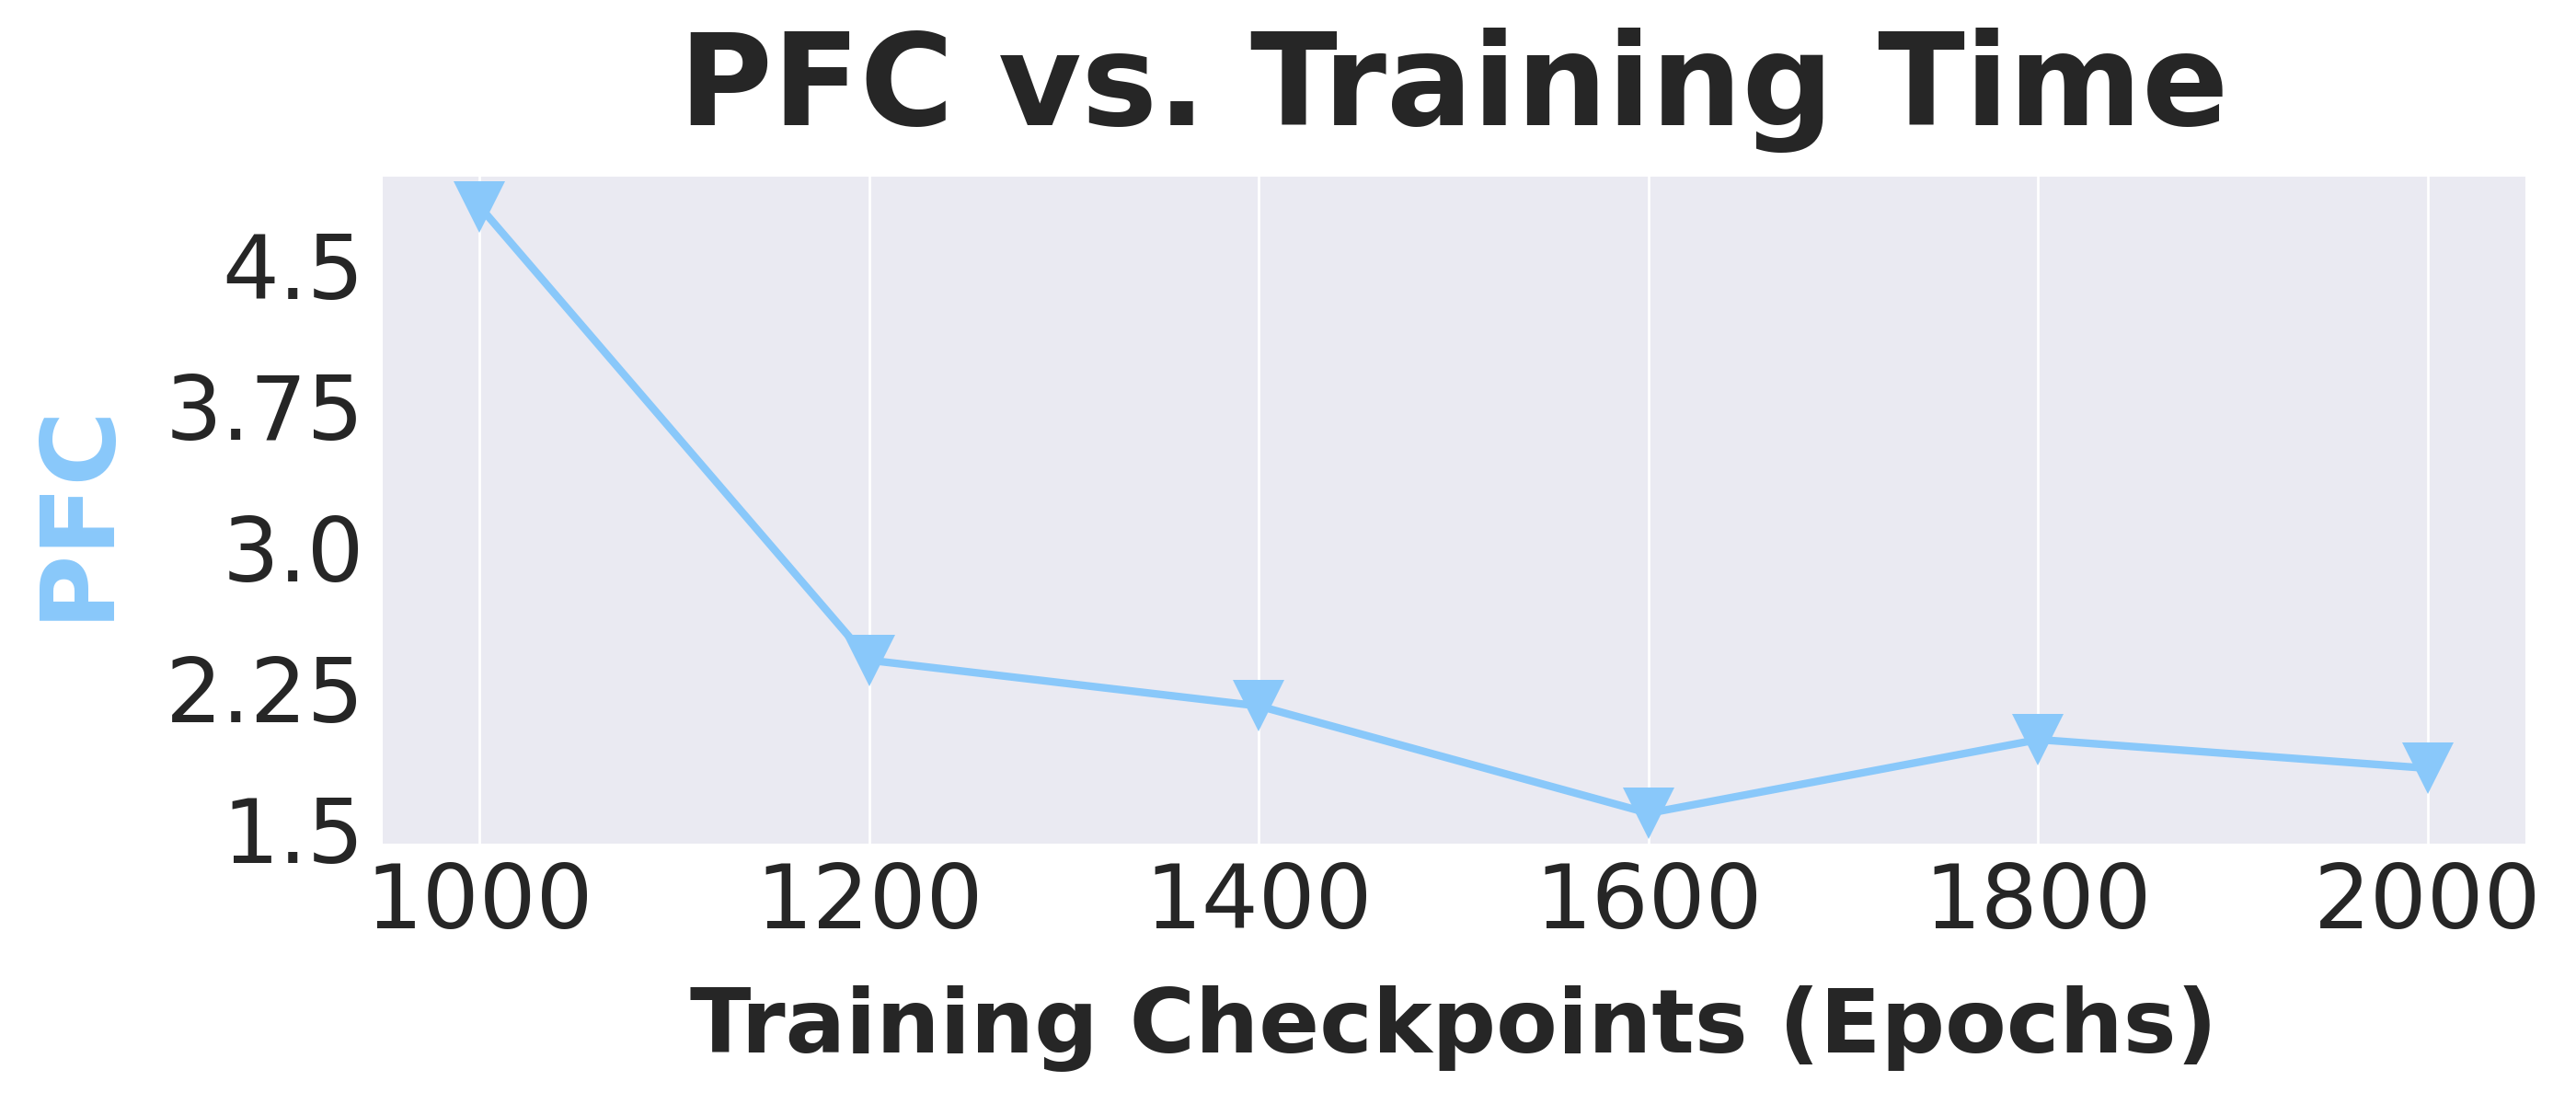
\includegraphics[width=\linewidth]{Figure7.png}
    \caption{PFC decreases throughout training.}
    \label{fig:7}
\end{figure}

\section{In-the-wild Music}
\label{sec:appendix_ood_music}

We use the below songs for our in-the-wild music demos:
\begin{itemize}
    \item \href{https://www.youtube.com/watch?v=S05hfsRbw3M}{Doja Cat - Woman}
    \item \href{https://www.youtube.com/watch?v=kJQP7kiw5Fk}{Luis Fonsi - Despacito ft. Daddy Yankee}
    \item \href{https://www.youtube.com/watch?v=MjCZfZfucEc}{ITZY - LOCO}
    \item \href{https://www.youtube.com/watch?v=x5c2iRHlAHA}{Saweetie - My Type}
    \item \href{https://www.youtube.com/watch?v=Xv9023cub0Y}{Rihanna - Only Girl (In The World)})
\end{itemize}

\section{Hyperparameters}

\begin{tabular}{c|c} 
 \hline
 Hyperparameter & Value \\
 \hline
 Optimizer & Adan~\cite{xie2022adan} \\ 

 Learning Rate & 4e-4 \\

 Diffusion Steps & 1000 \\

 $\beta$ schedule & cosine \\

 Motion Duration & 5 seconds\\

 Motion FPS & 30\\

 Motion Dimension & 151\\

 Classifier-Free Dropout & 0.25\\

 Num Heads & 8\\

 Num Layers & 8\\

 Transformer Dim & 512\\

 MLP Dim & 1024\\

 Dropout & 0.1\\

 EMA Steps & 1\\

 EMA Decay & 0.9999\\
 \hline
\end{tabular}

\section{Guidance Weight at Inference Time}
In our experiments, we find that dropping out the guidance at early denoising steps (i.e. set $w=0$ from step 1000 to step 800) further helps to increase diversity.
We perform this dropout for the version of our model sampled at $w=1$, dropping out 40\% of the steps.

\section{Memory-efficient Jukebox Implementation}
\label{sec:appendix_juke_mem}

Jukebox extraction implementations from previous work \cite{castellon2021codified,donahue2021sheet} are limited in memory efficiency (cannot load in the full model on a GPU with 16GB VRAM) and speed on short clips (performs inference as if the clip has full sequence length).

We improve upon these implementations and develop a new implementation that (1) improves memory efficiency two-fold and (2) speeds up extraction time 4x for 5-second clips.

\begin{itemize}
    \item For memory efficiency, we use \href{https://huggingface.co/docs/accelerate/v0.11.0/en/big_modeling}{HuggingFace Accelerate} to initialize the model on the ``meta'' device followed by loading in the checkpoint with CUDA, meaning that only half of the memory is used (using the traditional loading mechanism, PyTorch does not de-allocate the initial random weights allocated before the checkpoint is loaded in).
    \item For speed, we adapt the codebase to accept and perform inference on shorter clips.
    Our new implementation takes only $\sim\hspace{-3pt}5$ seconds for a 5-second clip on a Tesla T4 GPU.
\end{itemize}

These improvements make extracting representations from Jukebox more accessible to researchers and practitioners.

Additionally, to downsample to 30 FPS we use \textit{librosa}'s \href{https://librosa.org/doc/main/generated/librosa.resample.html}{resampling method} with ``fft'' as the resampling type to avoid unnecessary slowness.

We plan to release this new implementation together with our code release.

\section{Long-Form Generation}

Shown below is the pseudocode for long-form sampling.

\begin{lstlisting}[language=Python]
def long_generate():
    z = randn((batch, sequence, dim))
    half = z.shape[1] // 2
    for t in range(0, num_timesteps)[::-1]:
        # sample z from step t to step t-1
        z = p_sample(z, cond, t)
        # enforce constraint
        if t > 0:
            z[1:,:half] = z[:-1,half:]
    x = z
    return x
\end{lstlisting}

\section{Rigging}
In order to render generated dances in three dimensions for our \website, we export joint angle sequences to the FBX file format to be imported into Blender, which provides the final rendering. The character avatar used in all our renders except for those of dances from \textit{Bailando} is ``Y-Bot'', downloaded from Mixamo. Dances from \textit{Bailando} are rendered using ball-and-rod stick figures to ensure fair comparison, since dances are generated in Cartesian joint position space. Although inverse kinematic (IK) solutions are available, we sought to avoid the potential introduction of extraneous artifacts caused by poorly tuned IK, and instead rendered the joint positions directly. We perform no post-processing on model outputs.
\section{Extra Figures}
\begin{figure*}
    \centering
    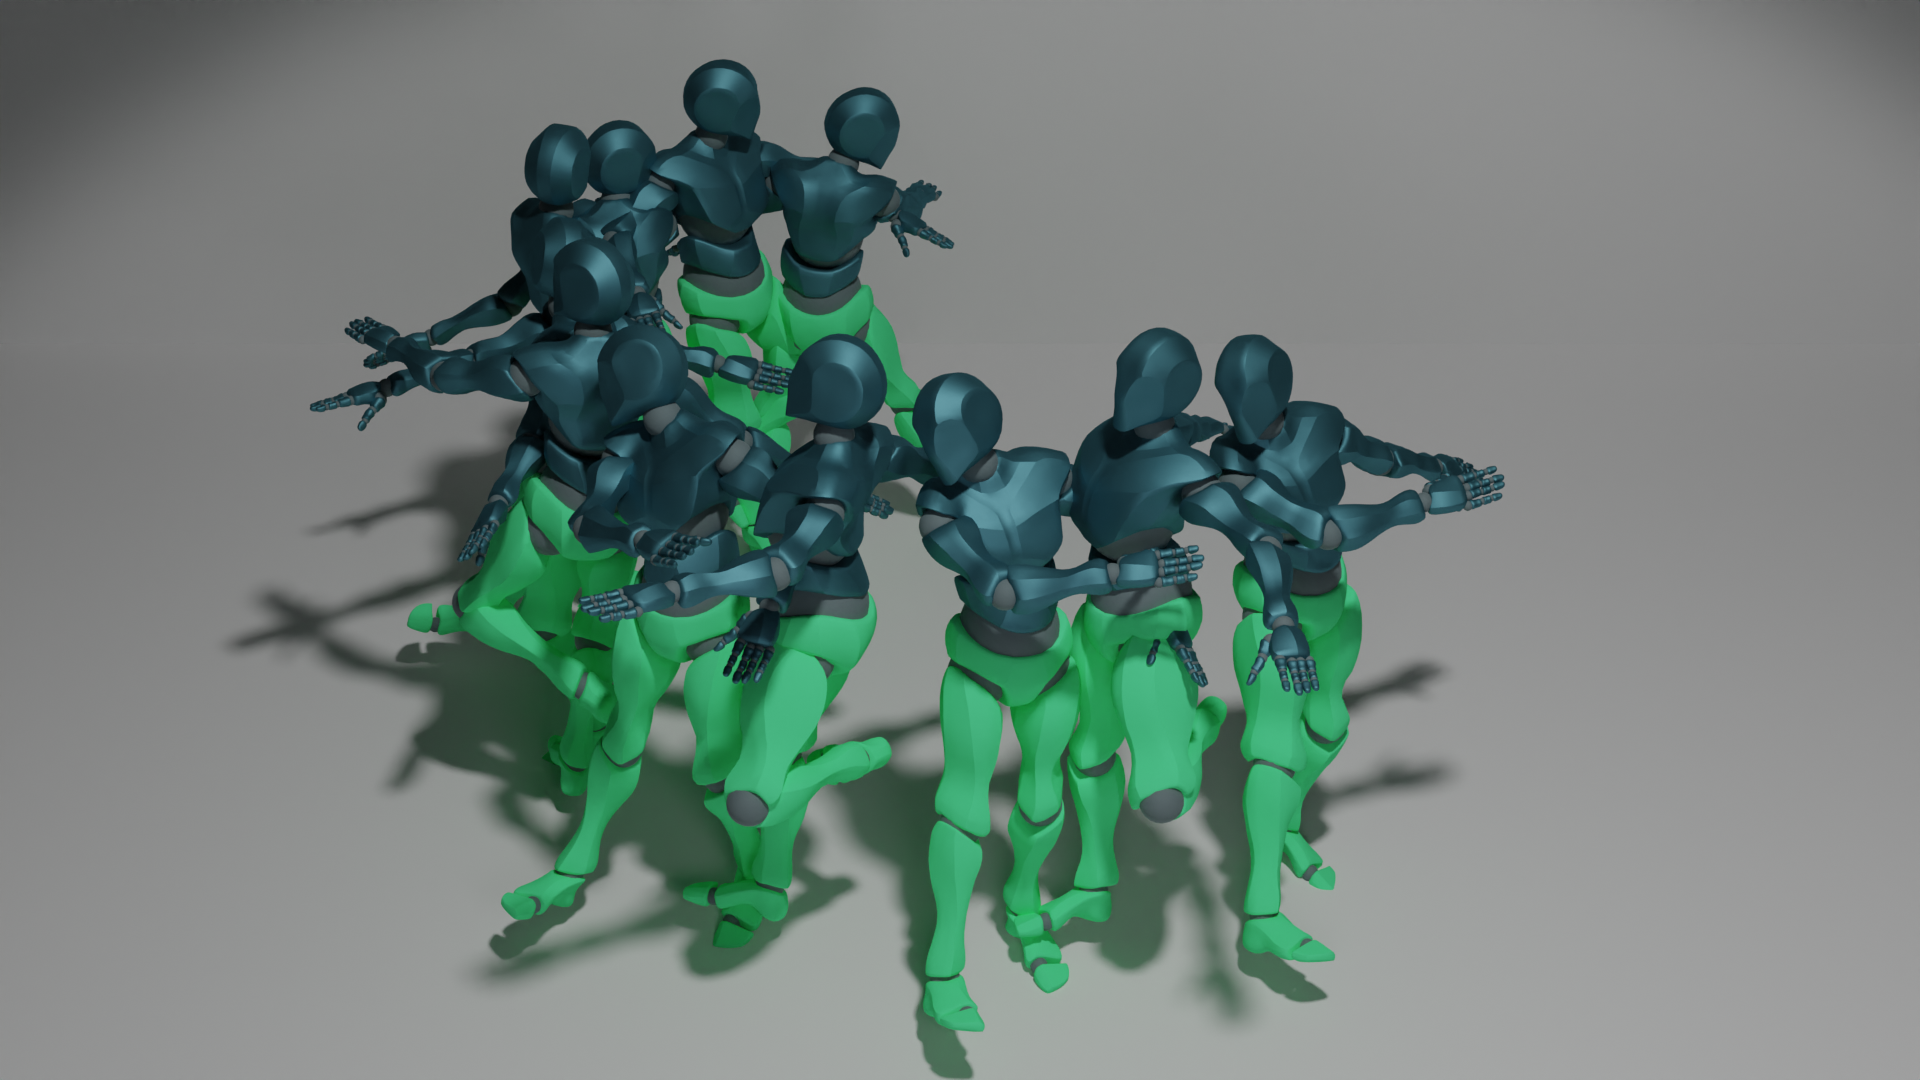
\includegraphics[width=0.9\linewidth]{Figure8.png}
    \caption{\textbf{Joint-wise Conditioning:} EDGE can generate upper body motion given a lower body motion constraint.}
    \label{fig:8}
\end{figure*}
\begin{figure*}
    \centering
    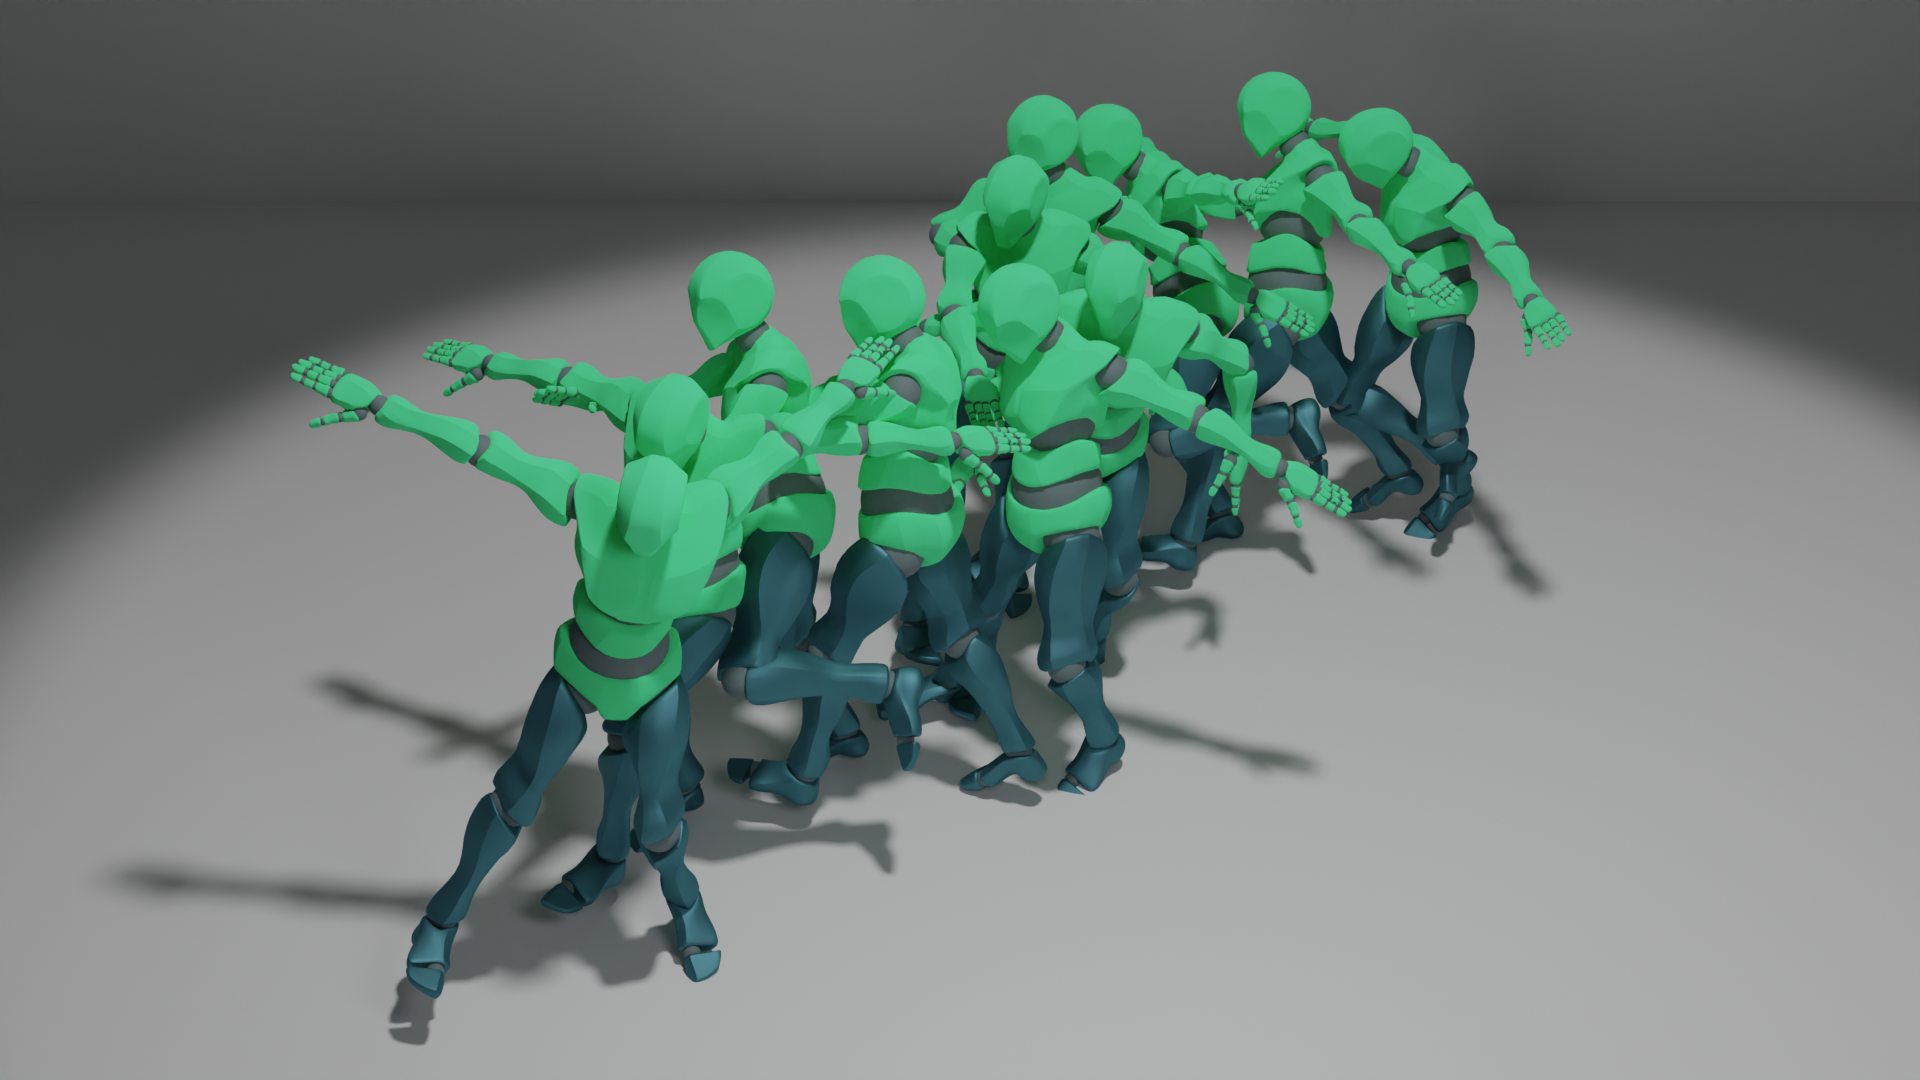
\includegraphics[width=0.9\linewidth]{Figure9.png}
    \caption{\textbf{Joint-wise Conditioning:} EDGE can generate lower body motion given an upper body motion constraint.}
    \label{fig:9}
\end{figure*}
\begin{figure*}
    \centering
    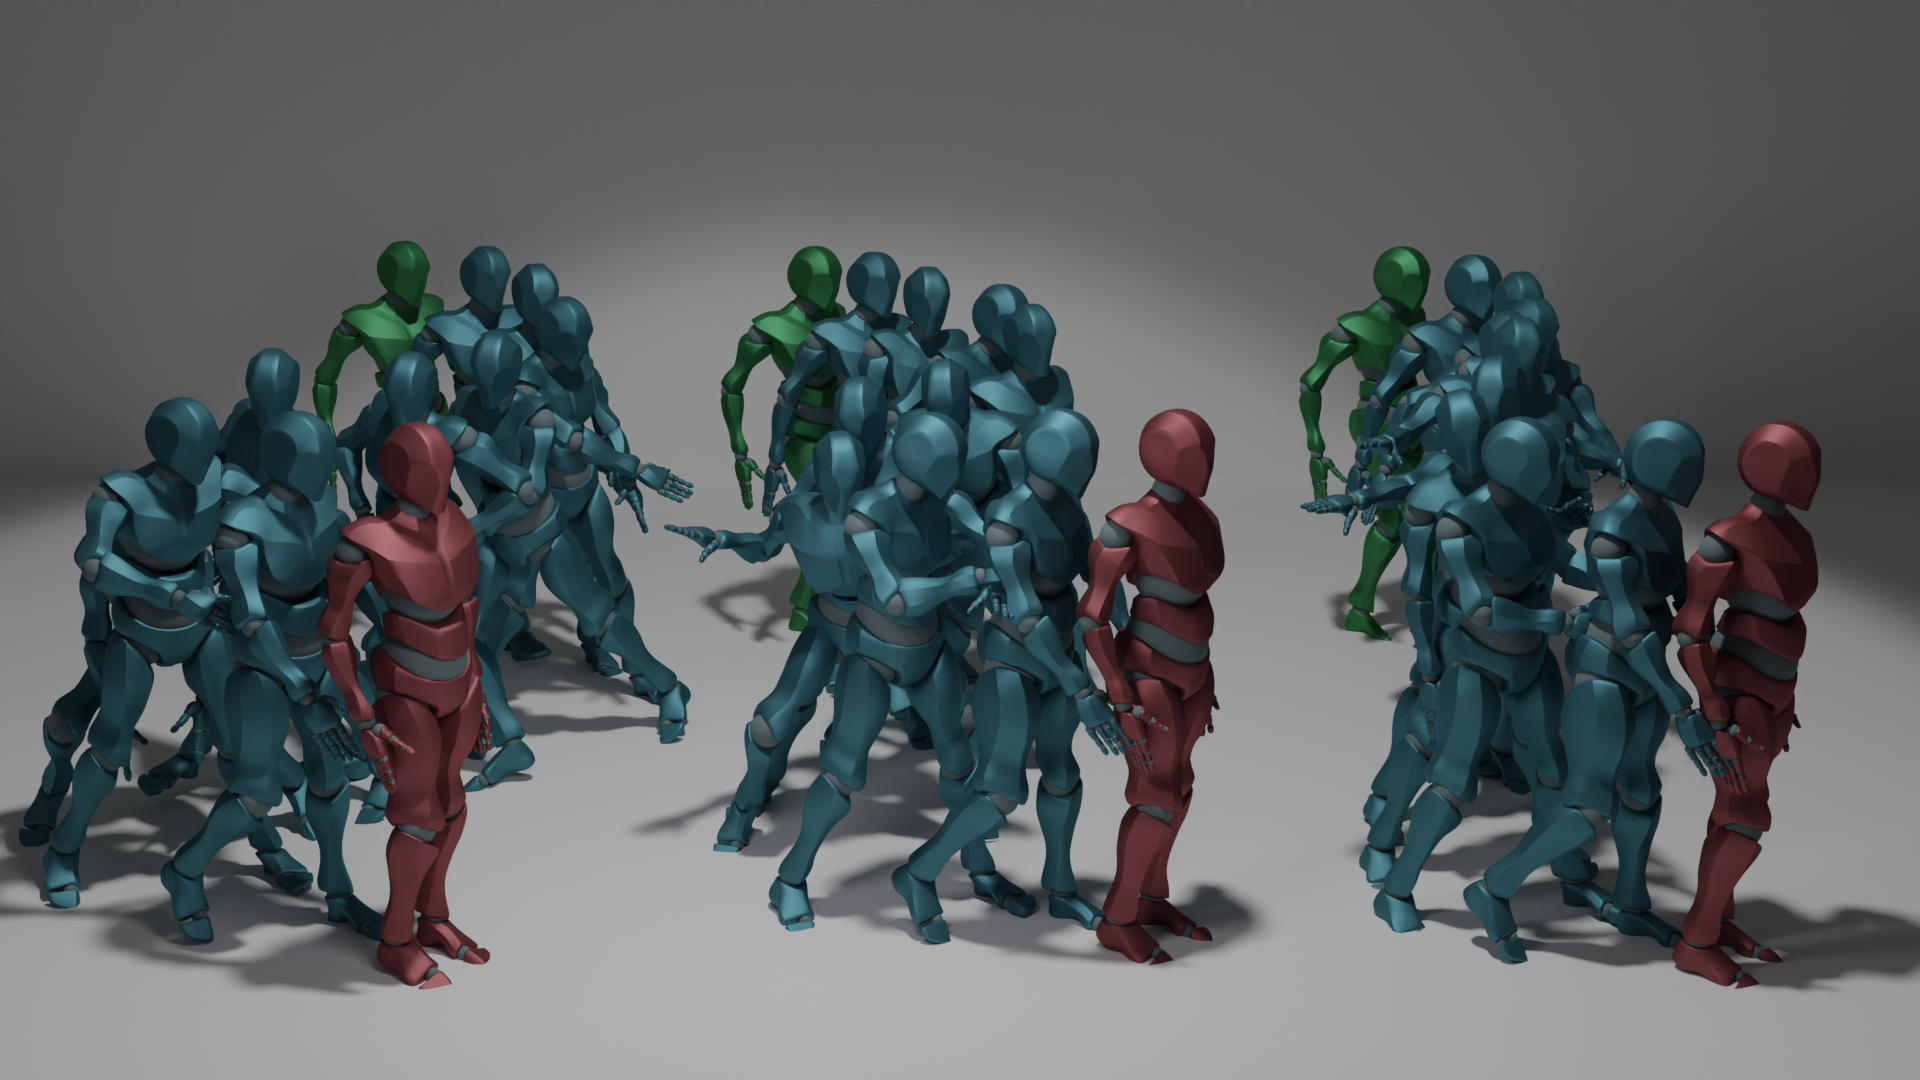
\includegraphics[width=0.9\linewidth]{Figure10.png}
    \caption{\textbf{Temporal Conditioning: In-Betweening} Given start and end poses, EDGE can generate diverse in-between dance sequences.}
    \label{fig:10}
\end{figure*}
\begin{figure*}
    \centering
    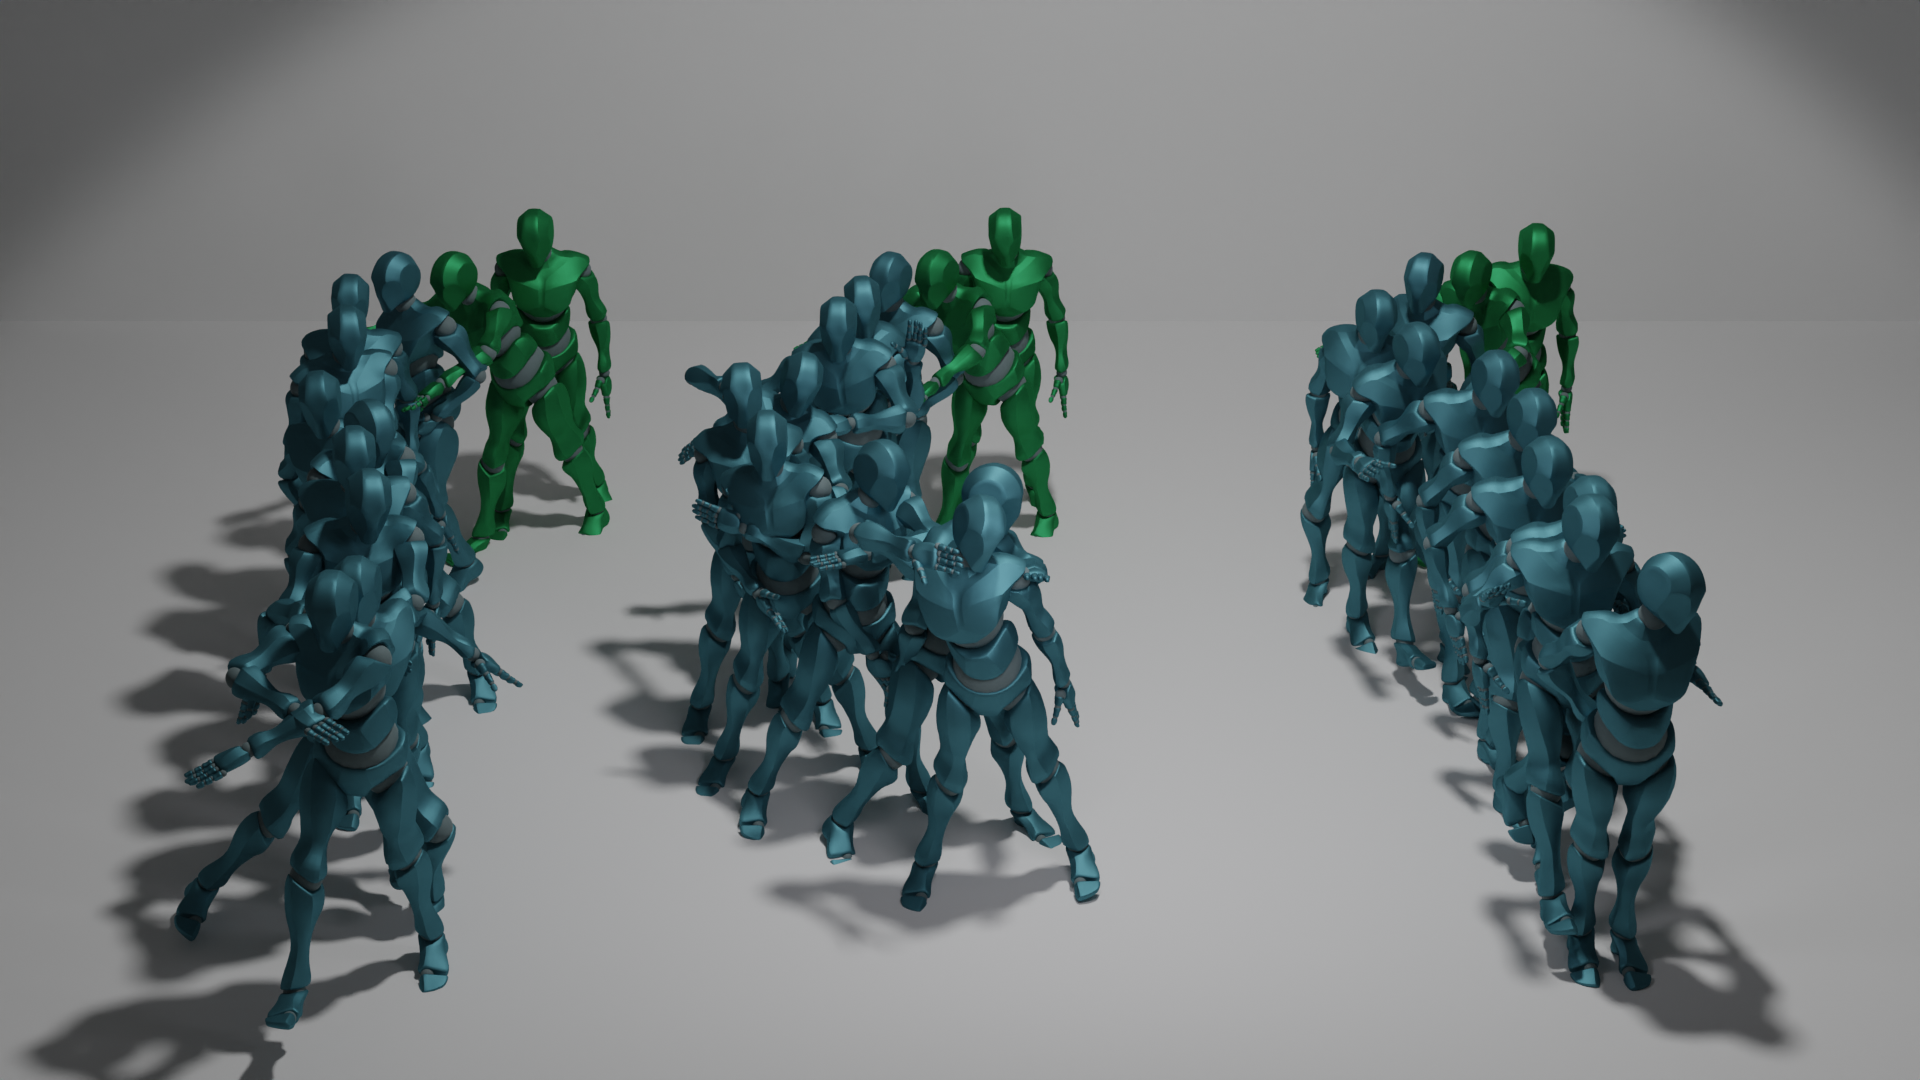
\includegraphics[width=0.9\linewidth]{Figure11.png}
    \caption{\textbf{Temporal Conditioning: Continuation} Given a seed motion, EDGE can continue the dance  in response to arbitrary music conditioning.}
    \label{fig:11}
\end{figure*}